\documentclass{tufte-book}

\hypersetup{colorlinks}% uncomment this line if you prefer colored hyperlinks (e.g., for onscreen viewing)

%%
% Book metadata
\title{Fucking ODE\\\noindent with fucking\\\noindent images}
\author[Aakash Ghosh]{Aakash Ghosh}
\publisher{Written in Pain}

%%
% If they're installed, use Bergamo and Chantilly from www.fontsite.com.
% They're clones of Bembo and Gill Sans, respectively.
%\IfFileExists{bergamo.sty}{\usepackage[osf]{bergamo}}{}% Bembo
%\IfFileExists{chantill.sty}{\usepackage{chantill}}{}% Gill Sans

%\usepackage{microtype}

%%
% For nicely typeset tabular material
\usepackage{booktabs}

%%
% For graphics / images
\usepackage{graphicx}
\setkeys{Gin}{width=\linewidth,totalheight=\textheight,keepaspectratio}
\graphicspath{{graphics/}}

% The fancyvrb package lets us customize the formatting of verbatim
% environments.  We use a slightly smaller font.
\usepackage{fancyvrb}
\fvset{fontsize=\normalsize}

%%
% Prints argument within hanging parentheses (i.e., parentheses that take
% up no horizontal space).  Useful in tabular environments.
\newcommand{\hangp}[1]{\makebox[0pt][r]{(}#1\makebox[0pt][l]{)}}

%%
% Prints an asterisk that takes up no horizontal space.
% Useful in tabular environments.
\newcommand{\hangstar}{\makebox[0pt][l]{*}}

%%
% Prints a trailing space in a smart way.
\usepackage{xspace}

%%
% Some shortcuts for Tufte's book titles.  The lowercase commands will
% produce the initials of the book title in italics.  The all-caps commands
% will print out the full title of the book in italics.
\newcommand{\vdqi}{\textit{VDQI}\xspace}
\newcommand{\ei}{\textit{EI}\xspace}
\newcommand{\ve}{\textit{VE}\xspace}
\newcommand{\be}{\textit{BE}\xspace}
\newcommand{\VDQI}{\textit{The Visual Display of Quantitative Information}\xspace}
\newcommand{\EI}{\textit{Envisioning Information}\xspace}
\newcommand{\VE}{\textit{Visual Explanations}\xspace}
\newcommand{\BE}{\textit{Beautiful Evidence}\xspace}

\newcommand{\TL}{Tufte-\LaTeX\xspace}

% Prints the month name (e.g., January) and the year (e.g., 2008)
\newcommand{\monthyear}{%
	\ifcase\month\or January\or February\or March\or April\or May\or June\or
	July\or August\or September\or October\or November\or
	December\fi\space\number\year
}


% Prints an epigraph and speaker in sans serif, all-caps type.
\newcommand{\openepigraph}[2]{%
	%\sffamily\fontsize{14}{16}\selectfont
	\begin{fullwidth}
	\sffamily\large
	\begin{doublespace}
	\noindent\allcaps{#1}\\% epigraph
	\noindent\allcaps{#2}% author
	\end{doublespace}
	\end{fullwidth}
}

% Inserts a blank page
\newcommand{\blankpage}{\newpage\hbox{}\thispagestyle{empty}\newpage}

\usepackage{units}

% Typesets the font size, leading, and measure in the form of 10/12x26 pc.
\newcommand{\measure}[3]{#1/#2$\times$\unit[#3]{pc}}

% Macros for typesetting the documentation
\newcommand{\hlred}[1]{\textcolor{Maroon}{#1}}% prints in red
\newcommand{\hangleft}[1]{\makebox[0pt][r]{#1}}
\newcommand{\hairsp}{\hspace{1pt}}% hair space
\newcommand{\hquad}{\hskip0.5em\relax}% half quad space
\newcommand{\TODO}{\textcolor{red}{\bf TODO!}\xspace}
\newcommand{\na}{\quad--}% used in tables for N/A cells
\providecommand{\XeLaTeX}{X\lower.5ex\hbox{\kern-0.15em\reflectbox{E}}\kern-0.1em\LaTeX}
\newcommand{\tXeLaTeX}{\XeLaTeX\index{XeLaTeX@\protect\XeLaTeX}}
% \index{\texttt{\textbackslash xyz}@\hangleft{\texttt{\textbackslash}}\texttt{xyz}}
\newcommand{\tuftebs}{\symbol{'134}}% a backslash in tt type in OT1/T1
\newcommand{\doccmdnoindex}[2][]{\texttt{\tuftebs#2}}% command name -- adds backslash automatically (and doesn't add cmd to the index)
\newcommand{\doccmddef}[2][]{%
	\hlred{\texttt{\tuftebs#2}}\label{cmd:#2}%
	\ifthenelse{\isempty{#1}}%
		{% add the command to the index
			\index{#2 command@\protect\hangleft{\texttt{\tuftebs}}\texttt{#2}}% command name
		}%
		{% add the command and package to the index
			\index{#2 command@\protect\hangleft{\texttt{\tuftebs}}\texttt{#2} (\texttt{#1} package)}% command name
			\index{#1 package@\texttt{#1} package}\index{packages!#1@\texttt{#1}}% package name
		}%
}% command name -- adds backslash automatically
\newcommand{\doccmd}[2][]{%
	\texttt{\tuftebs#2}%
	\ifthenelse{\isempty{#1}}%
		{% add the command to the index
			\index{#2 command@\protect\hangleft{\texttt{\tuftebs}}\texttt{#2}}% command name
		}%
		{% add the command and package to the index
			\index{#2 command@\protect\hangleft{\texttt{\tuftebs}}\texttt{#2} (\texttt{#1} package)}% command name
			\index{#1 package@\texttt{#1} package}\index{packages!#1@\texttt{#1}}% package name
		}%
}% command name -- adds backslash automatically
\newcommand{\docopt}[1]{\ensuremath{\langle}\textrm{\textit{#1}}\ensuremath{\rangle}}% optional command argument
\newcommand{\docarg}[1]{\textrm{\textit{#1}}}% (required) command argument
\newenvironment{docspec}{\begin{quotation}\ttfamily\parskip0pt\parindent0pt\ignorespaces}{\end{quotation}}% command specification environment
\newcommand{\docenv}[1]{\texttt{#1}\index{#1 environment@\texttt{#1} environment}\index{environments!#1@\texttt{#1}}}% environment name
\newcommand{\docenvdef}[1]{\hlred{\texttt{#1}}\label{env:#1}\index{#1 environment@\texttt{#1} environment}\index{environments!#1@\texttt{#1}}}% environment name
\newcommand{\docpkg}[1]{\texttt{#1}\index{#1 package@\texttt{#1} package}\index{packages!#1@\texttt{#1}}}% package name
\newcommand{\doccls}[1]{\texttt{#1}}% document class name
\newcommand{\docclsopt}[1]{\texttt{#1}\index{#1 class option@\texttt{#1} class option}\index{class options!#1@\texttt{#1}}}% document class option name
\newcommand{\docclsoptdef}[1]{\hlred{\texttt{#1}}\label{clsopt:#1}\index{#1 class option@\texttt{#1} class option}\index{class options!#1@\texttt{#1}}}% document class option name defined
\newcommand{\docmsg}[2]{\bigskip\begin{fullwidth}\noindent\ttfamily#1\end{fullwidth}\medskip\par\noindent#2}
\newcommand{\docfilehook}[2]{\texttt{#1}\index{file hooks!#2}\index{#1@\texttt{#1}}}
\newcommand{\doccounter}[1]{\texttt{#1}\index{#1 counter@\texttt{#1} counter}}

% Generates the index
\usepackage{makeidx}
\makeindex

% add numbers to chapters, sections, subsections
\setcounter{secnumdepth}{0}



\usepackage[most]{tcolorbox}


\newtheorem{theorem}{Theorem}
\newtheorem{definition}[theorem]{Definition}
\newtheorem{claim}[theorem]{Claim}
\newtheorem{proposition}[theorem]{Proposition}
\newtheorem{lemma}[theorem]{Lemma}
\newtheorem{corollary}[theorem]{Corollary}
\newtheorem{conjecture}[theorem]{Conjecture}
\newtheorem{observation}{Observation}
\newtheorem{example}{Example}
\newtheorem{remark}{Remark}



\setlength\parindent{0pt}


\begin{document}


% r.3 full title page
\maketitle


\tableofcontents

\mainmatter

















\chapter{Existance and uniqueness of solutions}
Everyone asks where solution, no one cares how solution :/
\begin{enumerate}
	\item $\mathbb D$: Domain, contains everything
\end{enumerate}

\begin{tcolorbox}[colback=red!5!white]
\textbf{IVP: }Let $D\subset \mathbb R\times \mathbb R^n$ be an open set and $f:\mathbb D\to \mathbb R^n$ be a function. The following is an \textbf{Initial value problem} or \textbf{IVP}:
$$\frac{dx}{dt}=f(x,t)\quad x(t_0)=x_0$$ 
\end{tcolorbox}

\begin{marginfigure}
	
\includegraphics{1.png}
\end{marginfigure}


\begin{tcolorbox}[colback=red!5!white]
\textbf{Solution: }A function $X$ on an interval is called the solution if 
\begin{enumerate}
	\item $X$ is differentiable and $X(t_0)=x_0$
	\item $(t,X(t))\in\mathbb D$ for all $t\in I$
	\item $\frac{d}{dt}X=f$
\end{enumerate}  
\end{tcolorbox}


\begin{tcolorbox}[colback=blue!8!white]
	$X$ is the solution of IVP iff:
	$$X(t)=x_0+\int_{t_0}^t f(s,X(s))ds$$
\end{tcolorbox}

\begin{tcolorbox}[colback=red!5!white]
	\textbf{Uniformly Lipschitz: }$f(t,x)$ is said to be uniformly Lipschitz w.r.t $t$ if for every $t$ there exists $L$ such that $|f(t,x)-f(t,y)|\leq L|x-y|$ for all $x,y$ such that $(t,x)$ and $(t,y)$ is in doamin. $L$ is called the Lipschitz constant.
\end{tcolorbox}


\begin{marginfigure}
	
\includegraphics{2.png}
\end{marginfigure}

\begin{tcolorbox}[colback=red!5!white]
	\textbf{Fixed Point: }$x$ is the fixed point of a map $T:\mathbb R^n\to\mathbb R^n$ if $Tx=x$
\end{tcolorbox}

\begin{tcolorbox}[colback=red!5!white]
	\textbf{Contraction: }$T:\mathbb R^n\to\mathbb R^n$ is a contraction if there exists $0\leq c<1$ such that $|Tx-Ty|\leq c|x-y|$ for all pairs $x,y$
\end{tcolorbox}

\begin{tcolorbox}[colback=blue!8!white]
	\textbf{Banch Fixed Point Theorem }: Every contraction has an unique fixed point.
\end{tcolorbox}

\begin{tcolorbox}[colback=blue!8!white]
	\textbf{Picard Lindelof theorem}: For an IVP, let $c,r$ be chosen such that $[t_0-c,t_0+c]\times\overline{B_r(x_0)}\subset\mathbb D$. Let $f$ be uniformly Lipschitz with constant $L$. Let $M$ be the maximum value of $f$ in $[t_0-c,t_0+c]\times\overline{B_r(x_0)}$. Define $h:=\min\{c,r/M,1/L\}$(the $1/L$ condition can be dropped). There exists a unique solution to the IVP $X:(t_0-h,t_0+h)\to\\overline{B_r(x_0)}$
\end{tcolorbox}

\begin{marginfigure}
	
\includegraphics{3.png}
\end{marginfigure}

\begin{tcolorbox}[colback=blue!8!white]
	\textbf{Maximal Interval of a solution }: Let $X:I\to\mathbb R^n$ be the solution of IVP. Then there exists a maximal interval of existance of $X$ as a solution.
\end{tcolorbox}


\begin{tcolorbox}[colback=blue!8!white]
	\textbf{Maximal Interval of a solution }: Let $X:(a,b)\to\mathbb{R}^n$ be a solution of IVP. $[t_0,b)$ is the right maximal interval of solution if for every compact $K$ in $\mathbb D$ there exists $t\in[t_0,b)$ such that $(t,X(t))\notin K$
\end{tcolorbox}

\begin{tcolorbox}[colback=blue!8!white]
	\textbf{Maximal Interval of a solution }: Let $f$ be continuous and let $(a,b)$ be the maximal interval of existance of $X$ as a solution. Then:
	\begin{enumerate}
		\item If $\partial \mathbb D\ne\phi,b<\infty$ and if $\lim_{t\to b^{-}}X(t)$ exists then $(b,\lim_{t\to b^{-1}}X(t))\in\partial \mathbb D$
		\item If $\partial \mathbb D=\phi$ and $b<\infty$ then $$\limsup_{t\to b^{-}}||X(t)||=\infty$$
	\end{enumerate}
\end{tcolorbox}


\begin{marginfigure}
	
\includegraphics{4.png}
\end{marginfigure}


\begin{tcolorbox}[colback=red!5!white]
	\textbf{Global Solution: }Let $D=I\times \mathbb R^n$, where $I$ is an open interval. We say a global solution exists if a solution exists on $I$.
\end{tcolorbox}

\begin{tcolorbox}[colback=blue!8!white]
	\textbf{Existance of Global solution }: Let $I$ be an open interval on $\mathbb R$. Let $f$ be such that 
	$$|f(x,t)|\leq M(t)+|x|N(t)$$
	for some non negative continuous $M,N$. Then the maximal interval of existance of every solution in $I$(i.e. every solution can be extended to a global solution)
\end{tcolorbox}
\begin{marginfigure}
	
\includegraphics{5.png}
\end{marginfigure}


\begin{tcolorbox}[colback=green!8!white]
	A maximal solution exists if $f$ is uniformly Lipschitz on $I$.
\end{tcolorbox}

\begin{tcolorbox}[colback=green!8!white]
	Let $I\subset\mathbb R$ be open interval and let $A:I\to \mathbb{R}^{n\times n}$ be a linear map. Let $b:I\to\mathbb R^n$  be continuous. Then a global solution exists for the following IVP:
	$$X'(t)=A(t)X(t)+b(t)\quad X(t_0)=x_0$$ 
\end{tcolorbox}
\begin{figure*}
	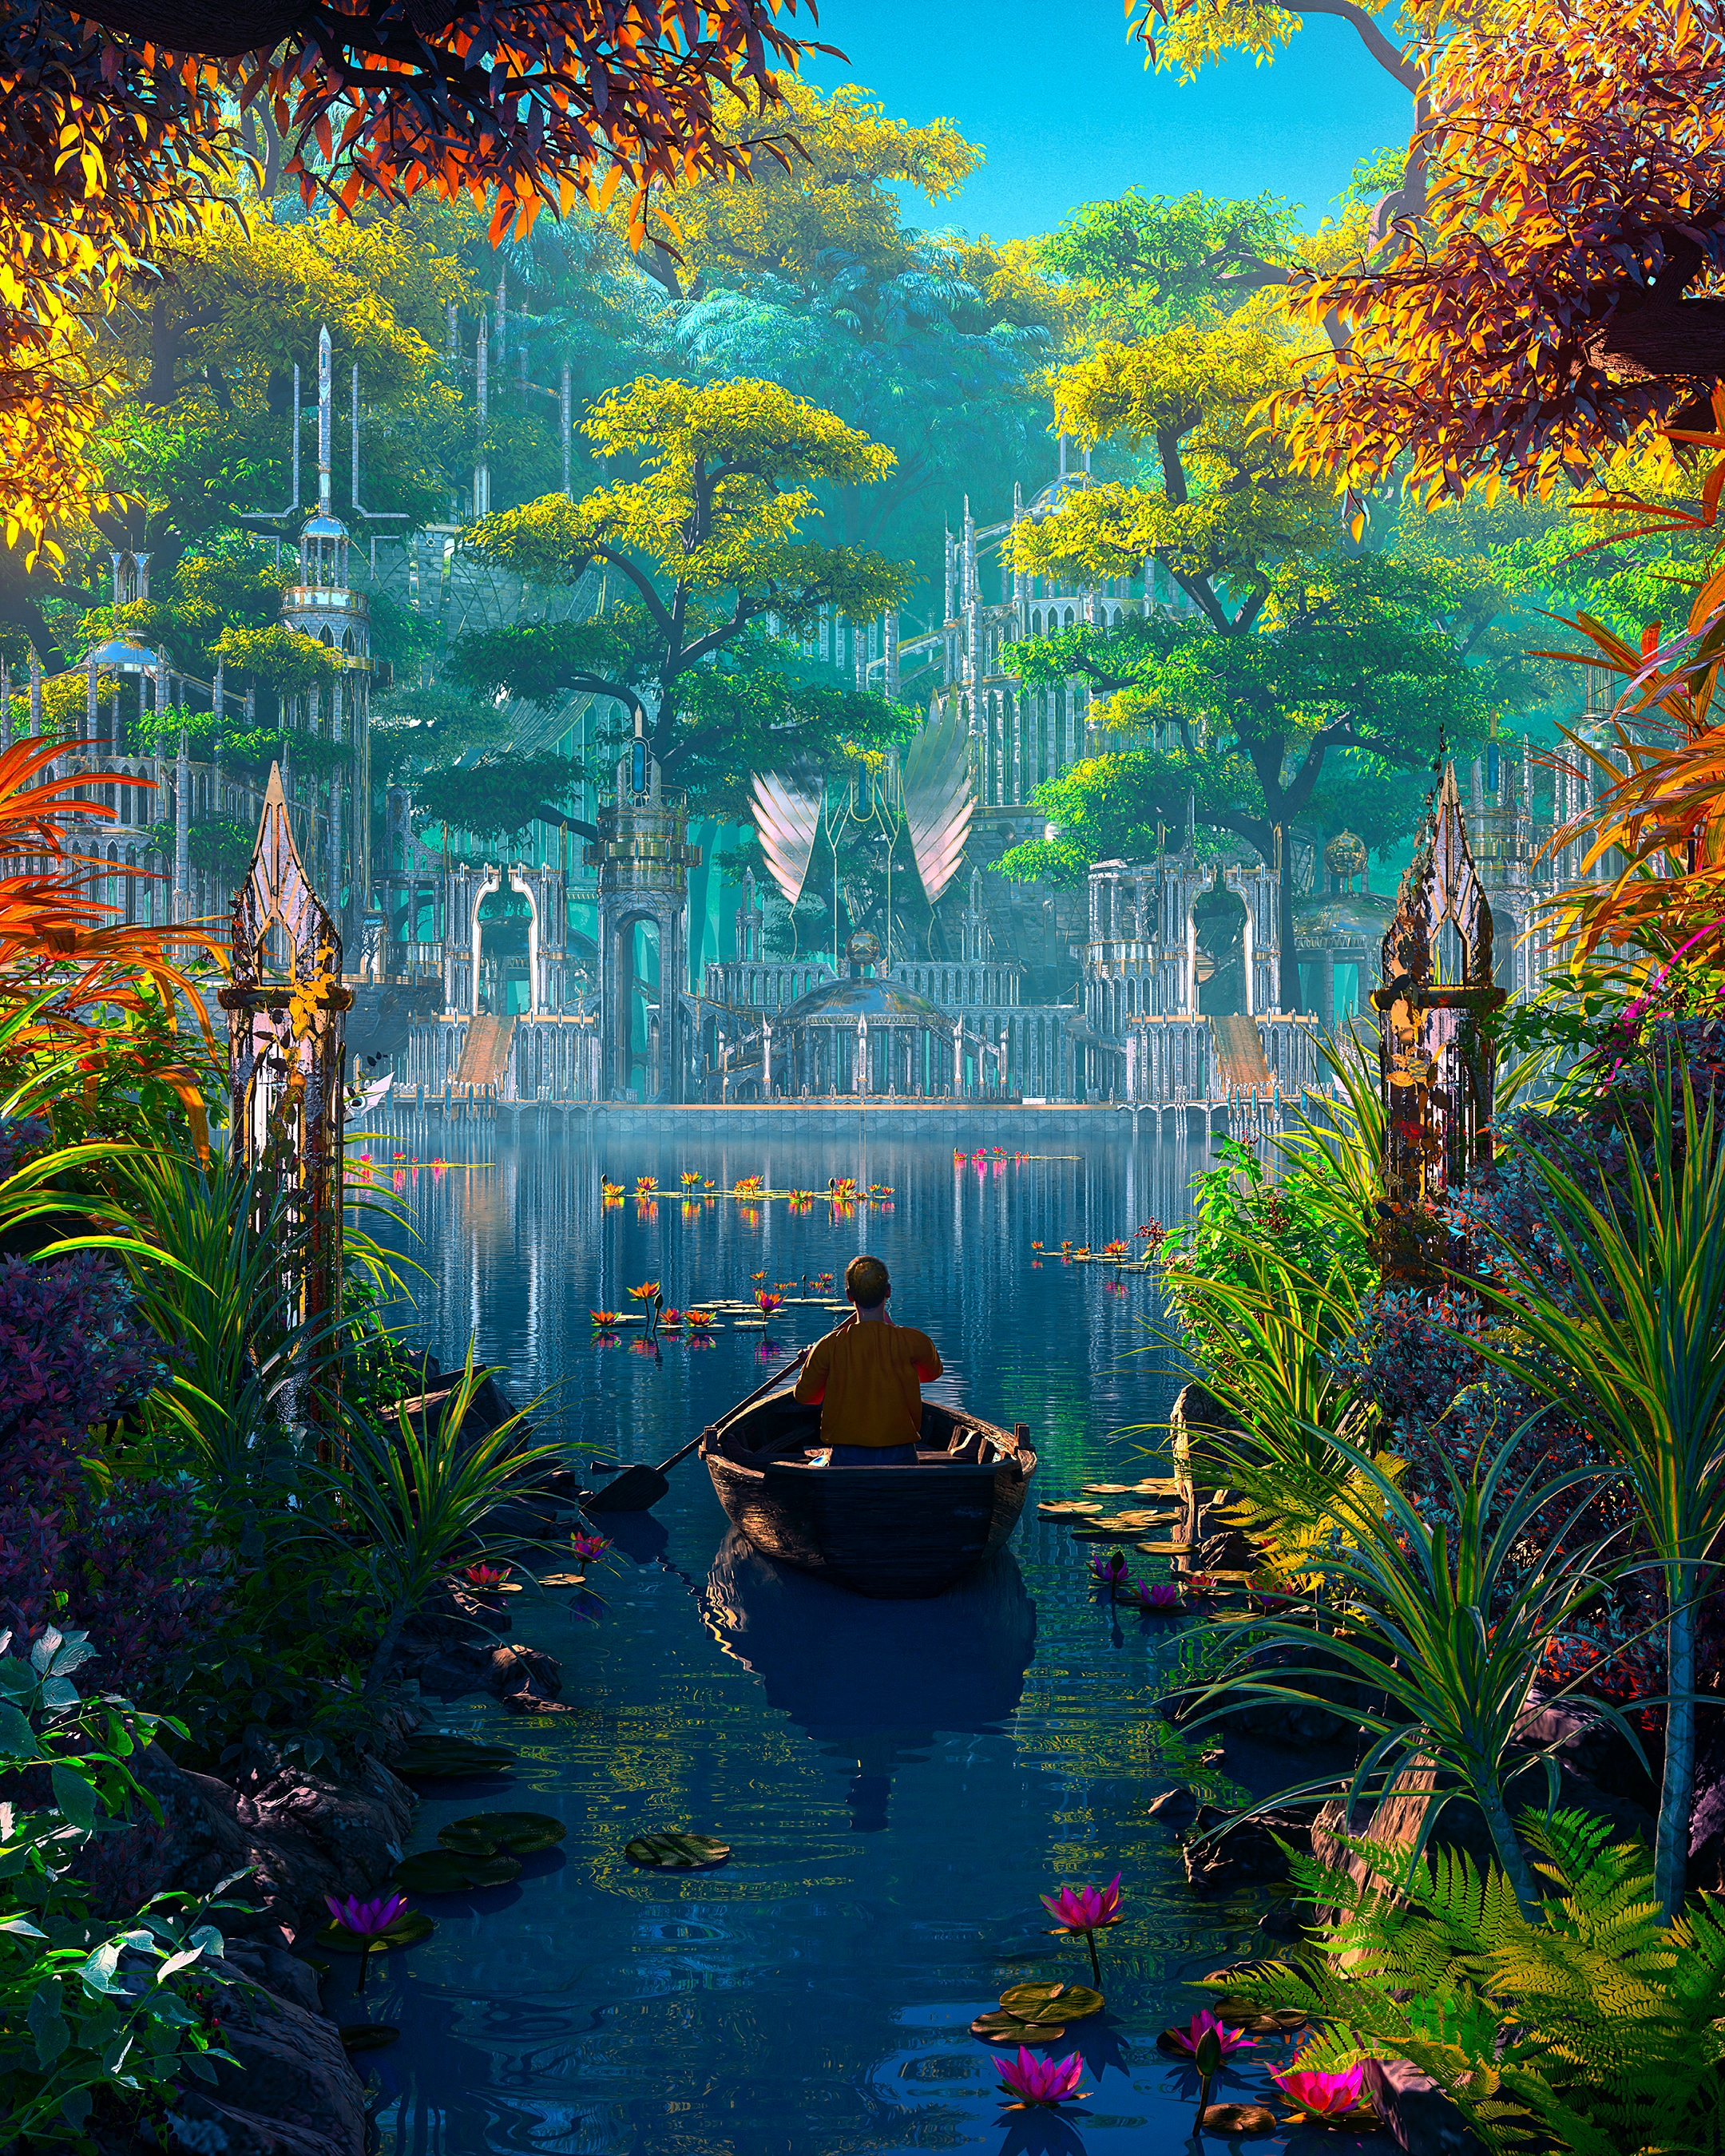
\includegraphics[width=\textwidth]{1-1.jpg}
\end{figure*}

\chapter{Linear Systems of ODE}
An IVP is a linear system if there exits a linear transformation $A$ such that 
$$x'(t)=Ax(t)$$
[i.e $f$ is a linear transformation]

\begin{tcolorbox}[colback=red!5!white]
	\textbf{$e^A$: }: For a linear transformation $T:\mathbb R^n\to\mathbb R^n$ we define $e^A=\sum_{i=0}^\infty \frac{A^n}{n!}$
\end{tcolorbox}
\begin{marginfigure}
	
\includegraphics{6.png}
\end{marginfigure}
\begin{tcolorbox}[colback=blue!8!white]
	$$\frac{d}{dt}e^{At}=Ae^{At}$$
	$$AB=BA\Rightarrow e^{A+B}=e^Ae^B$$
\end{tcolorbox}


\begin{tcolorbox}[colback=blue!8!white]
	\textbf{Fundamental theorem of Linear systems }: Let $A\in M_n(\mathbb R)$. Then the IVP $X'(t)=AX(t),X(0)=X_0$ has the solution:
	$$X(t)=e^{At}X_0$$
\end{tcolorbox}
\begin{tcolorbox}[colback=blue!8!white]
	Let $A\in M_n(\mathbb R)$. Then the IVP $X'(t)=AX(t)+b(t),X(0)=X_0$ has the solution:
	$$X(t)=e^{At}\left(\int_0^t e^{-At}b(t)dt+X_0\right)$$
\end{tcolorbox}
\begin{marginfigure}
	
\includegraphics{7.png}
\end{marginfigure}
Problem-solving strat for $e^A$ calculation:
\begin{enumerate}
	\item Break $A$ in $B$ and $C$ such that $B$ is diagonal and $C$ is upper triangular( or in some othere form such that $B$ is diagonal and $C$ is nillpotent with $BC+CB$)
	\item Use the fact that $e^A=e^{B+C}e^Be^C$
\end{enumerate}
\begin{figure*}
	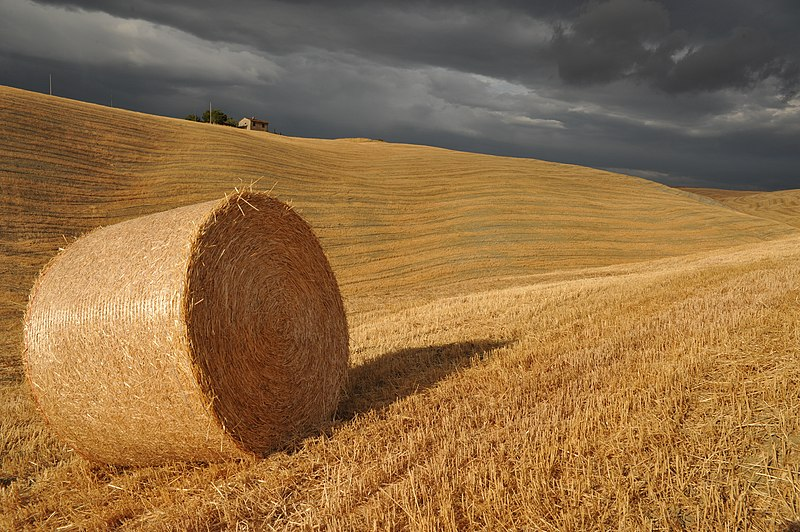
\includegraphics{2-2.jpg}
\end{figure*}

\chapter{Stability of solutions}
\section{Phase Portraits}
THERE ARE SUPPOSED TO BE PICTURES HERE> REVIEW PHASE PORTRAITS BEFORE EXAM
\begin{marginfigure}
	
\includegraphics{8.png}
\end{marginfigure}
\begin{tcolorbox}[colback=red!5!white]
	A linear system is said to have 
	\begin{enumerate}
		\item A \textbf{saddle} at the origin if $A\sim\begin{bmatrix}
			\lambda &0\\0 &\mu
		\end{bmatrix},\lambda<0<\mu$
		\item A \textbf{mode} at the origin if $A\sim\begin{bmatrix}
			\lambda &0\\0 &\mu
		\end{bmatrix},\lambda\mu>0$ or  $A\sim\begin{bmatrix}
			\lambda &1\\0 &\lambda
		\end{bmatrix}$
		\item A \textbf{focus} at the origin if $A\sim\begin{bmatrix}
			a &b\\-b &a
		\end{bmatrix},a\ne0$
		\item A \textbf{center} at the origin if $A\sim\begin{bmatrix}
			0 &b\\-b &0
		\end{bmatrix}$
	\end{enumerate}
\end{tcolorbox}
\begin{tcolorbox}[colback=red!5!white]
	\textbf{Autonomous system: }An IVP is an autonomous system if $f$ is independent of $t$. 
\end{tcolorbox}

\begin{marginfigure}
	
\includegraphics{9.png}
\end{marginfigure}

\begin{tcolorbox}[colback=red!5!white]
	\textbf{Equilibrium point: }$x_0$ is an equilibrium point of autonomous system $f$ if $f(x_0)=0$
\end{tcolorbox}
\begin{tcolorbox}[colback=red!5!white]
	\textbf{Flow: }Let $\phi(t,y_0)$ be the solution of IVP $x'=f(x),x(0)=y_0$. Then the map defined by $\phi_t(x)=\phi(t,x)$ is called the flow of the IVP. 
\end{tcolorbox}
\begin{tcolorbox}
	\textbf{Properties of flow}:
	\begin{enumerate}
		\item $\phi_0(x)=x$
		\item $\phi_s\phi_t(x)=\phi_{t+s}(x)$
		\item $\phi_{-t}\phi_t(x)=x$
	\end{enumerate}
\end{tcolorbox}

\begin{marginfigure}
	
\includegraphics{10.png}
\end{marginfigure}

\begin{tcolorbox}[colback=red!5!white]
	Consider an autonomous nonlinear dynamical system
$$
\dot{x}=f(x(t)), \quad x(0)=x_0,
$$
Suppose $f$ has an equilibrium at $x_e$ so that $f\left(x_e\right)=0$ then
\begin{enumerate}
	\item This equilibrium is said to be \textbf{Lyapunov stable}, if, for every $\epsilon>0$, there exists a $\delta>0$ such that, if $\left\|x(0)-x_e\right\|<\delta$, then for every $t \geq 0$ we have $\left\|x(t)-x_e\right\|<\epsilon$.
	\item The equilibrium of the above system is said to be \textbf{asymptotically stable} if it is Lyapunov stable and there exists $\delta>0$ such that if $\left\|x(0)-x_e\right\|<\delta$, then $\lim _{t \rightarrow \infty}\left\|x(t)-x_e\right\|=0$.
\end{enumerate}
\end{tcolorbox}


\begin{tcolorbox}[colback=red!5!white]
	Let $f$ and $V$ be continuous functions on the domain. Define:
	$$\dot{V}(x)=\nabla V(x)\cdot f(x)$$
\end{tcolorbox}

\begin{tcolorbox}[colback=blue!8!white]
	$$\dot V(x)=\frac{d}{dt}\Bigg|_{t=0}V\circ \phi_t(x)$$
\end{tcolorbox}

\begin{marginfigure}
	
\includegraphics{11.png}
\end{marginfigure}

\begin{tcolorbox}[colback=blue!8!white]
	Consider an autonomous nonlinear dynamical system
$$
\dot{x}=f(x(t)), \quad x(0)=x_0,
$$
Suppose $f$ has an equilibrium at $x_e$ and let $V$ be a differentiable function with $V(x_0)=0, V(x)>0\forall x\ne x_0$. Then:
\begin{enumerate}
	\item If $\dot V(x)\leq 0\forall x\in E$ then $x_e$ is stable.
	\item If $\dot V(x)< 0\forall x\in E\setminus\{x_e\}$ then $x_0$ is asymptotically stable.
	\item If $\dot V(x)> 0\forall x\in E\setminus\{x_e\}$ then $x_e$ is unstable.
\end{enumerate}
\end{tcolorbox}

Problem solving strat:
\begin{enumerate}
	\item $V$ is our potential candidate for potential function
	\item Try $V=\sum c_ix_i^2$
	\item If 2 doesn't work try $V=\sum c_ix^{\alpha_i}$
	\item If 3 doesn't work, pray
\end{enumerate}

\begin{figure*}
	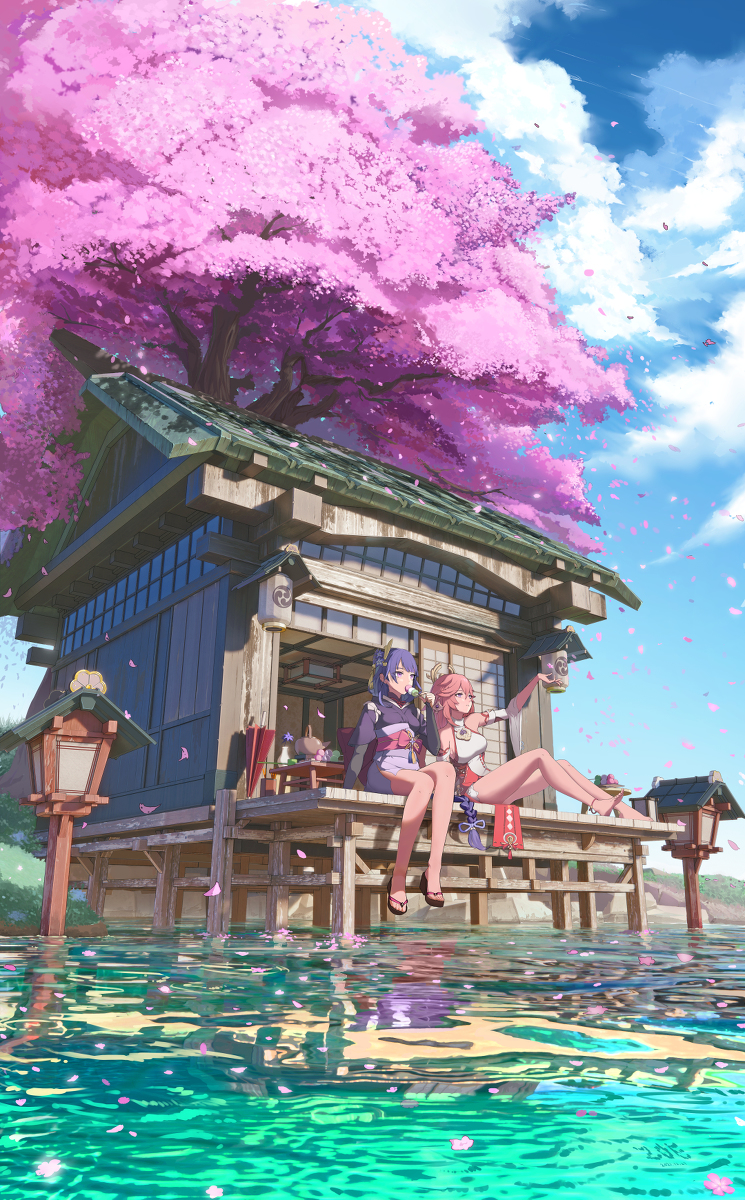
\includegraphics[width=0\textwidth]{3-3.jpg}
\end{figure*}


\backmatter


\bibliography{sample-handout}z
\bibliographystyle{plainnat}


\end{document}

